\subsection{Distributed Denial of Service (DDoS)}
\label{subsec:03_ddos}

% Introduction describing the base of such attacks
A DDoS (Distributed Denial of Service) attack has become a popular way to cripple a server of an institution or a private person and exposed to be an immense threat to the Internet. However, how is it possible for attackers to execute such attacks? The current internet design has its purpose of moving packets from a source to a known destination. The network itself minimally forwards all packages at minimal cost and generally outsources the complexity, including security, transport reliability and quality of service to the sender and receiver of the package. This concept has been called the end-to-end paradigm. As no intermediary entity will step in, a party (either sender or receiver) can damage its opposition by using different attack possibilities such as IP Spoofing or the aforementioned DDoS attack \cite{Mirkovic2004}. By faking the source address in the header of a packet, the sender can hide its identity. This security issue is called IP Spoofing \cite{Cloudflare2019}. As described in \citet{Mirkovic2004} following security issues raise opportunities of attacks:
\begin{itemize}
    \item Limited internet resources: Every host or services has hardware limitations that users may consume.
    \item Highly interdependent internet security: No matter how secure a host may be configured, DDoS attacks always depend on the security of others within the Internet.
    \item No collocation of intelligence and resources: The intermediate network has plentiful resources, as they forward package at minimal costs.  In contrast, the end networks only invest in as much bandwidth as they planned to use for their services.
    \item No enforcement of accountability: As described above, attackers can escape from accountability by using IP Spoofing mechanisms.
    \item Distribution of control: In a world of a distributed network, such as the Internet, multiple networks participate in that network. Each one of them has different security mechanisms. No global control entity can define a security policy or standard.
\end{itemize}
% TODO Additional reasons

% Explaining DDoS
By deploying multiple attacking entities, attackers using DDoS try to overflood a service and prevent others the use of that service. More precisely, they send a stream of packets to the victims, which consume the hardware resources and therefore make it unavailable for legitimate clients to access the service. Another popular way for an attacker is to send malformed packets to shut down the availability of the service. Those packets confuse the web application or some protocols on the victims' hardware and force the server to reboot. There are probably some additional possibilities to shut down services on the internet. Such attack possibilities will be discovered first when they have been exploited in a significant attack. The procedure of a DDoS attack is split into the following phases: An attacker recruits multiple agents (clients) into which the attacker injects malicious code. Attackers often hide the identity of infected clients by using IP Spoofing mechanisms \cite{Mirkovic2004}.

% TODO Difference DoS and DDoS?

% TODO Motivation behind DDoS
Multiple incentives exist to attack clients using DDoS attacks. Unfortunately, the main goal of such an attack is to damage the selected victim. The motives may be found in prestige (gaining respect within the hacker community when attacking popular websites), personal grudges, material gain meaning to attack competitors, any political reasons or simply blackmailing others \cite{Mirkovic2004}.

% TODO generalize possibilities of mitigation strategies

Various companies (known from other services) currently offer DDoS protection services, such as Cloudflare or Akami, and its number is increasing \cite{Pras2016}. For all solutions, a third party DDoS Protection Service (DPS) provider is required, resulting in extra costs, as the analysis performs in the cloud \cite{Rodrigues2017}.

% TODO DOTS (DDoS Open Threat Signaling) an IETF proposal
% TODO probably explain Gladius?

In the following sections, various approaches to mitigating DDoS attacks are illustrated.

% TODO ordering of subsubsections?

\subsubsection{DDos Mitigation with Smart Contracts}
This concept investigates a possibility to mitigate a DDoS attack in a fully decentralized manner using smart contracts. An architecture to do so will be illustrated within this section to create an automated DDoS mitigation system \cite{Rodrigues2017}.

As described in \ref{subsec:02_smart_contracts} a smart contract is a software that is made to help contracts being able to execute and verify on its own. To do so, there has to be an infrastructure that implements, verifies and enforces the negotiation of those smart contracts by using particular computer protocols and that runs fully decentralized. As you know from \ref{subsec:02_blockchain}, a blockchain ensures permanent storage and provides obstacles to manipulate content and is thus an ideal infrastructure for smart contracts.

% Proposed System Architecture
 % TODO describing architecture
\begin{figure}[ht]
  \begin{center}
  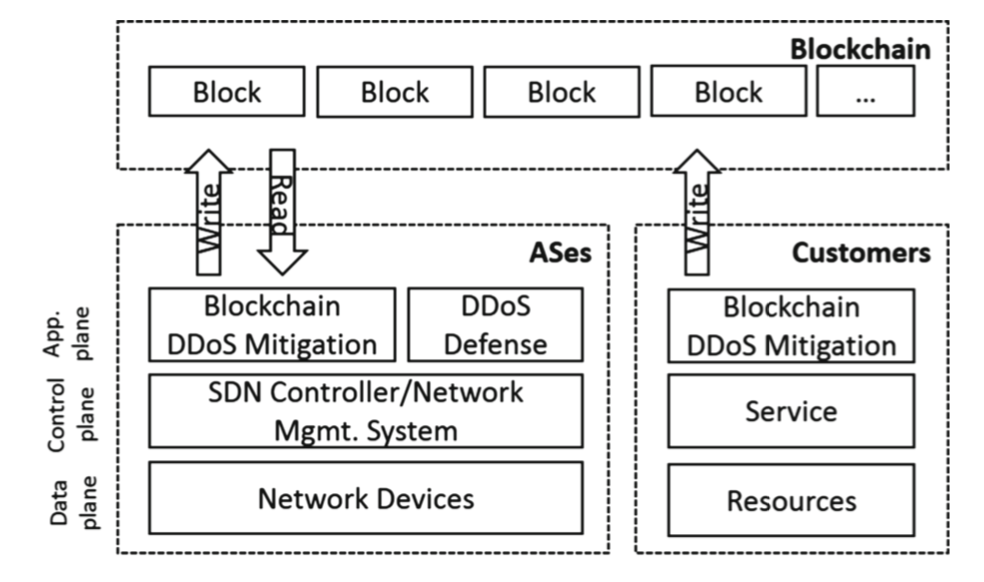
\includegraphics[scale=0.6]{Talk7/img/ddos/collaborative_ddos_mitigation_system_architecture}
  \end{center}
  \caption{System Architecture}
  \label{system_architecture}
\end{figure}

% TODO conclusion of this architecture


\subsubsection{Mitigation-as-a-service in cooperative network defenses}
% \cite{Mannhart2018}
% TODO introduction about cooperative network defneses?
When collaboratively countering DDoS attacks various Autonomous Systems (AS) are involved. As soon as a target AS detects an attack, the target requests to all participating AS's to mitigate the current attack. Subsequent, a mitigator AS, which is responsible for the range being attacked then either accepts or declines the mitigation request. By using a proof-of-mitigation the completion of the mitigation has to be confirmed and the target can pay the mitigator. As this proof-of-mitigation has to satisfy aspects of timeliness, tamper-evidence, and reproducibility this proof has to be executed automatically during the existing time-window \cite{Mannhart2018}. Additionally, any user interaction has to be excluded to ensure efficiency. Various approaches creating such proof will be described and discussed in this section.

\paragraph{Marketplace of Mitigation VNFs}
\begin{figure}[ht]
  \begin{center}
  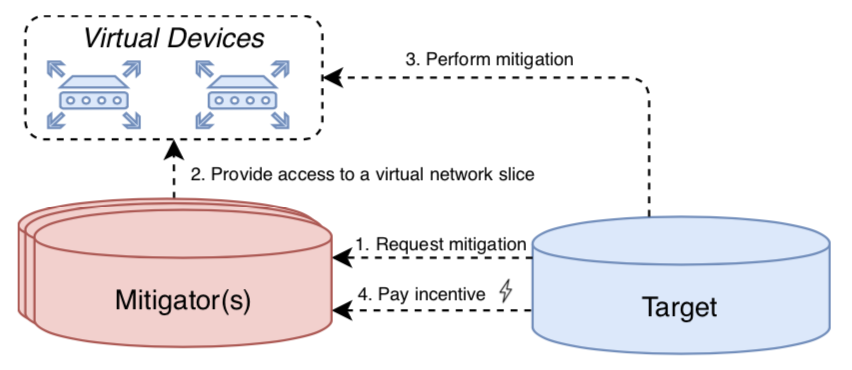
\includegraphics[scale=0.6]{Talk7/img/ddos/cooperative_network_marketplace_vnfs}
  \end{center}
  \caption{Marketplace of Mitigation VNFs}
  \label{ddos_marketplace_vnf}
\end{figure}
% TODO

\paragraph{Trusted Computing}
\begin{figure}[ht]
  \begin{center}
  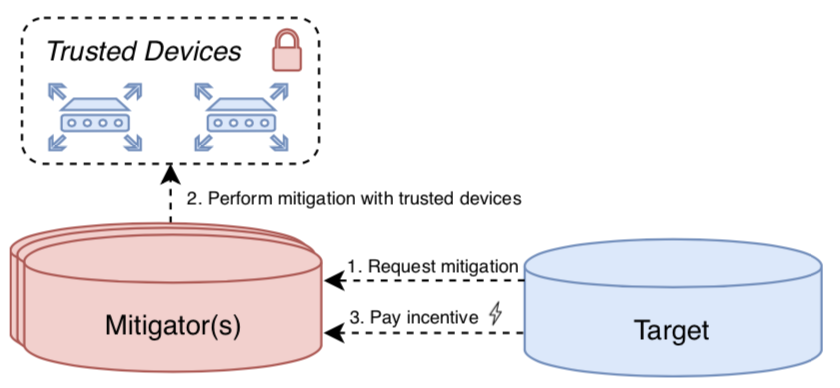
\includegraphics[scale=0.6]{Talk7/img/ddos/cooperative_network_trusted_computing}
  \end{center}
  \caption{Trusted computing}
  \label{ddos_trusted_computing}
\end{figure}
% TODO

\paragraph{Secure logging}
\begin{figure}[ht]
  \begin{center}
  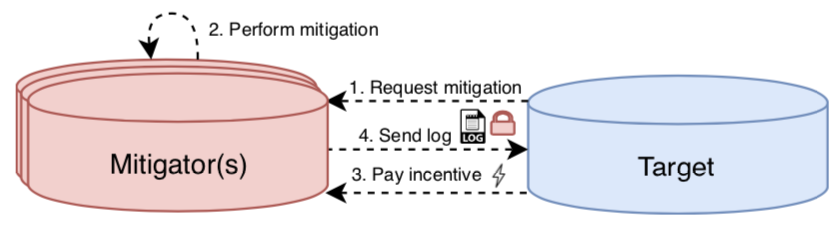
\includegraphics[scale=0.6]{Talk7/img/ddos/cooperative_network_secure_logging}
  \end{center}
  \caption{Secure logging}
  \label{ddos_secure_logging}
\end{figure}
% TODO

\paragraph{Network Slicing}
\begin{figure}[ht]
  \begin{center}
  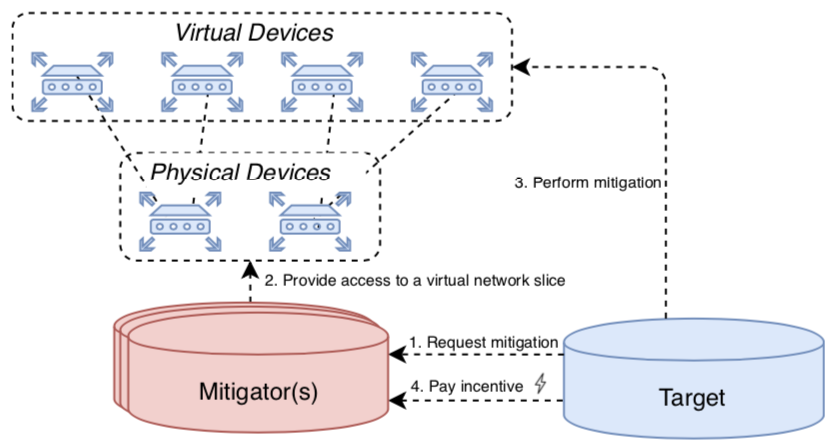
\includegraphics[scale=0.6]{Talk7/img/ddos/cooperative_network_network_slicing}
  \end{center}
  \caption{Network Slicing}
  \label{ddos_network_slicing}
\end{figure}
% TODO

% Final considerations of this paper

\subsubsection{Blockchain Signaling System (BloSS)}
% \cite{Rodrigues2019}

\subsubsection{Multi domain DDoS Mitgiation based on blockchains}
% \cite{Rodrigues2017a}
